\chapter{算法设计}

\section{问题描述}
对于给定一个以自然句子表示的即席查询$s$,共包含$l$个单词$\{w_1,w_2,\cdots,\\w_l\}$,本文研究的目标是建立一个
视频检索系统,即从$n$个未被标注的视频集$\{v_1,v_2,\cdots,v_n\}$中搜索出与该查询相关的视频。问题的关键是构建
一个跨模态的相似度函数$f(s,v) \in \mathbf{R}$,使得相关的句子视频对$(s,v^+)$的相似度比不相关的句子视频对$(s,v^-)$
更大。相应地,在查询结果中相关的视频$v^+$会排在不相关的视频$v^-$的视频前。设$\mathbf{s}$和$\mathbf{v}$是查询与视频
在公共空间的向量化表示,则跨模态的相似度由余弦相似度得到:
\begin{equation}
    \label{eq:cosine-sim}
    \begin{aligned}
        f(s,v) := \frac{\mathbf{s}^T\mathbf{v}}{\left\| \mathbf{s} \right\| \cdot \left\| \mathbf{v} \right\|}
    \end{aligned}
\end{equation}

本研究着眼于查询表示学习,即由查询$s$获得在公共空间的向量$\mathbf{s}$,而视频可以像之前的工作一样由深度卷积网络得到
的特征或者概念向量表示。

\section{查询表示学习}
本研究是建立在W2VV~\cite{dong2018predicting}模型的基础上,W2VV模型原本是用在图像描述或者视频描述的检索任务上,
共包含两个子网络,即一个句子编码网络,把一个句子向量化和一个转换网络,将句子向量转换到视觉特征空间中,如图\ref{fig:model1}所示。本研究对W2VV做如下改进:
\begin{itemize}
    \item 使用一个更好的句子编码策略。

    \item 使用一个更好的特征融合策略。

    \item 使用一个更好的目标函数用于模型训练。
\end{itemize}

\begin{figure*}[tbh!]
    \centering
    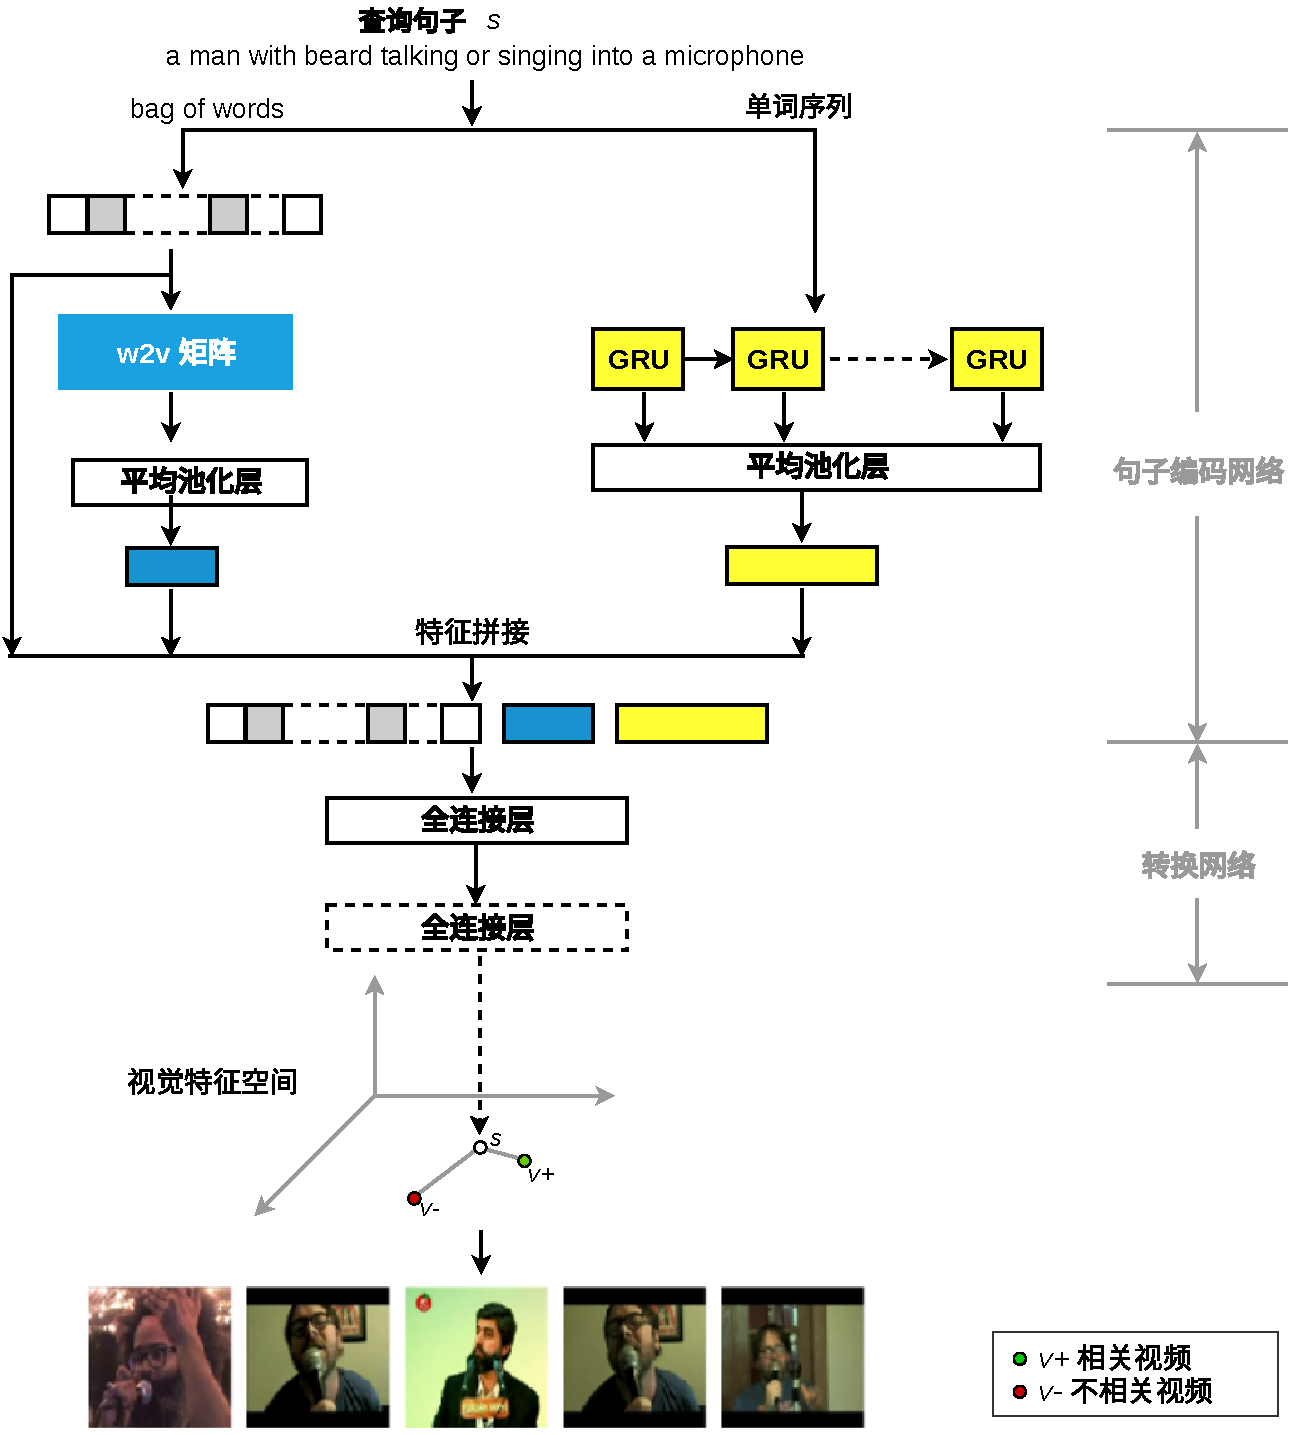
\includegraphics[width=\linewidth]{figures/model1}
    \caption[模型1]{这是模型1}
    \label{fig:model1}
\end{figure*}

\begin{figure*}[tbh!]
    \centering
    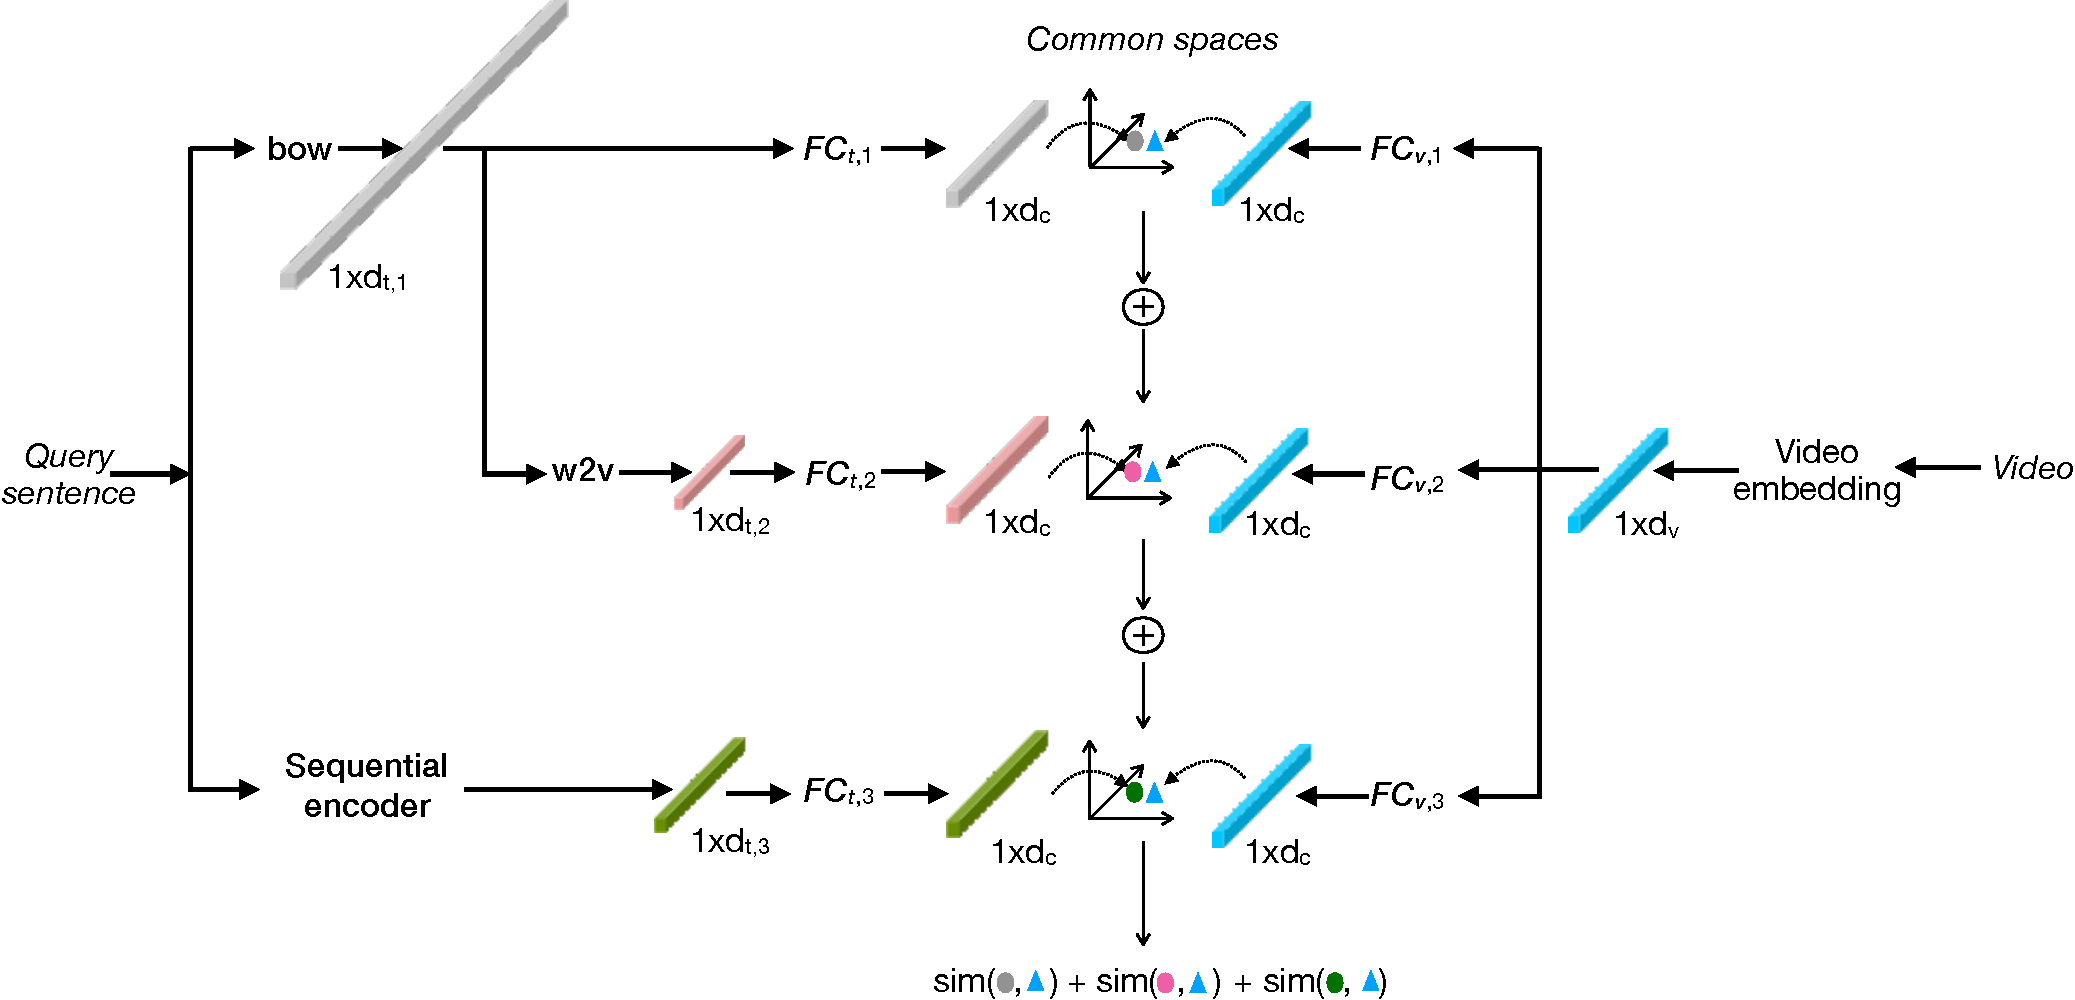
\includegraphics[width=\linewidth]{figures/model2}
    \caption[模型2]{这是模型2}
    \label{fig:model2}
\end{figure*}

\subsection{句子编码网络}
对于给定的一个句子$s$, 本研究同时使用三种编码技术对$s$进行向量化表示,即bag-of-words(bow),word2vec(w2v)词嵌入和
基于RNN的序列建模技术。对于bow编码技术,句子$s$的向量可以由如下式子得到:
\begin{equation}
    \label{eq:bow}
    \begin{aligned}
        \bm{\mathbf{bow}}(s) := (c(w_1,s),c(w_2,s),\cdots,c(w_m,s))
    \end{aligned}
\end{equation}
$c(w,s)$计算特定单词$w$在句子$s$中出现的次数,$m$表示给定词典的单词数量,本研究使用的词典由在训练数据中出现不少于5次
的单词组成,并且根据NLTK去掉其中的停用词。

对于一个给定的预训练w2v模型,用$\bm{\mathbf{e}}(w)$表示特定单词$w$的语义词嵌入向量,则w2v编码技术使用平均池化操作得到句子的向量:
\begin{equation}
    \label{eq:w2v}
    \begin{aligned}
        \bm{\mathbf{w2v}}(s) := \frac{1}{l}\sum^l_{i=1}e(w_i)
    \end{aligned}
\end{equation}
本研究使用一个500维的使用3000万张Flickr图像的英文标签训练的w2v模型~\cite{dong2018predicting},共支持超过170万个常见的单词向量化。

和W2VV相似,本研究同样使用Gated recurrent units(GRUs)~\cite{cho2014learning}作为序列模型对句子进行编码。GRU在特定的$t$时刻的输入
是句子中第$t$个单词的词嵌入向量,设为$\bm{\mathbf{e}}(w_t)$。该向量是从一个词嵌入矩阵$W_e$中对应的单词的词嵌入向量得到的。而GRU的输出,设为$h_t$
是通过联合当前词向量$\bm{\mathbf{e}}(w_t)$和GRU之前时刻的输出向量$h_{t-1}$由如下式子得到:
\begin{equation}
    \label{eq:gru}
    \begin{aligned}
        & z_t = \sigma_g(W_z e(w_t) + U_z h_{t-1} + b_z), \\
        & r_t = \sigma_g(W_r e(w_t) + U_r h_{t-1} + b_r), \\
        & \widetilde{h_t} = \sigma_h(W_h e(w_t) + U_h (r_t \circ h_{t-1}) + b_h), \\
        & h_t = (1-z_t) \circ h_{t-1} + z_t \circ \widetilde{h_t},
    \end{aligned}
\end{equation}
其中$z_t$ 和$r_t$表示在$t$时刻的更新门向量和重置门向量,$W$,$U$和$b$表示门的仿射转换参数,每个门输出前带有一个特定的激活函数,其中
$\sigma_g$表示sigmoid函数,$\sigma_h$表示双曲正切函数,操作$\circ$为两个向量的哈达玛积。

对于基于GRU的句子编码,W2VV只取最后时刻的输出向量,即$h_l$,而本研究通过对所有时刻的平均池化操作考虑所有的中间时刻的输出状态,即:
\begin{equation}
    \label{eq:gru-mean}
    \begin{aligned}
        \bm{\mathbf{gru}}(s) := \frac{1}{l}\sum^l_{i=1}h_i
    \end{aligned}
\end{equation}
对于GRU词典,与bow词典类似,但是GRU词典还包含停用词,因为它们在自然语句中含有有意义的上下文信息。

对于多种编码方式(bow, w2v, GRU)对句子进行编码,本文使用两种策略对这些编码方式进行融合,即:
\begin{itemize}
    \item W2VV++:使用与W2VV相同的方式,即向量拼接融合,即$\bm{\mathbf{ms}}(s)=[\bm{\mathbf{bow}}(s);\bm{\mathbf{w2v}}(s);\bm{\mathbf{gru}}(s)]$。本文将这种方式的模型称为W2VV++。

    \item TEE:三种编码方式互相独立,分别与视频向量。本文将这种方式的模型称为text encoding ensemble(TEE)。
\end{itemize}

\subsection{转换网络}
转换网络用于将之前的网络输出进行非线性仿射变换,即对于W2VV++模型,将$\bm{\mathbf{ms}}(s)$进行转换,对于TEE模型,分别对$\bm{\mathbf{bow}}(s)$,$\bm{\mathbf{w2v}}(s)$和$\bm{\mathbf{gru}}(s)$进行转换,
把文本编码得到的向量转换到一个公共空间,得到向量$\bm{\mathbf{s}}$,使得句子与视频的相关性可以由公式\ref{eq:cosine-sim}进行计算。
本文使用$k$层全连接层实现该转换网络。以W2VV++模型得到的文本编码向量$\bm{\mathbf{ms}}(s)$为例,对转换网络进行描述。第一层全连接层
的输出向量$\bm{\mathbf{fc_1}}(s)$由作用在向量$\bm{\mathbf{ms}}(s)$的仿射变换得到,即:
\begin{equation}
    \label{eq:fc-1}
    \begin{aligned}
        \bm{\mathbf{fc_1}}(s) = \sigma(A_1\bm{\mathbf{ms}}(s) + b_1)
    \end{aligned}
\end{equation}
其中$A_1$和$b_1$分别是全连接层的权重和偏移,$\sigma$是增强网络非线性的激活函数,本研究默认的激活函数是双曲正切函数。转换网络的剩余的全连接层计算如下公式:
\begin{equation}
    \label{eq:fc-k}
    \begin{aligned}
        \bm{\mathbf{fc_i}}(s) = \sigma(A_i\bm{\mathbf{fc_{i-1}}}(s) + b_i), i=2,...,k.
    \end{aligned}
\end{equation}
本研究的句子编码网络和转换网络是端到端地进行训练的,把网络的所有可学习的参数$\{W_z,U_z,b_z,W_r,U_r,b_r,W_h,U_h,b_h,W_e,A_1,b_1,\cdots,A_k,b_k\}$表示成$\theta$,相应地,相似度函数参数表示为$f(s,v;\theta)$。


\section{视频特征表示}
正如前文所言,本研究的目标在于查询表示学习,因此,对于视频的表示,本文简单地使用最先进的深度卷积网络通过过采样的方式提取视觉特征,
并且使用平均池化的操作获得视频的特征表示,如图\ref{fig:video-cnn-feat}所示。本文使用两个深度卷积网络模型进行视频的特征提取:
ResNeXt-101~\cite{xie2017aggregated}和ResNet-152~\cite{he2016deep}。对于每个模型,本文选择模型的分类层输出作为特征,维度为2048维。
对于给定一个视频,本研究以0.5秒为间隔对视频的帧进行均匀采样。每张采样的图像的大小调整为$256\times256$,然后以$224\times224$大小
的窗口对该图像与其水平翻转得到的图像的四个角和中央进行裁剪,得到该图像的10张子图,这10张子图分别经过卷积网络提取特征并且进行
平均池化操作,得到该图像的特征表示。相应地,2048维的视频特征由图像特征进行平均池化得到。为了方便表示,本文将使用$ResNeXt$和$Resnet$
表示经过这两种卷积网络得到的视频特征,$ResNeXt$-$Resnet$表示这两种特征进行拼接得到的4096维的视频特征。

原则上,本研究的模型可以使用任何的视频特征表示,包括概念特征向量~\cite{markatopoulou2017query,lu2016event,merler2012semantic}和3D卷积网络特征~\cite{mithun2018learning}。

\begin{figure*}[tbh!]
    \centering
    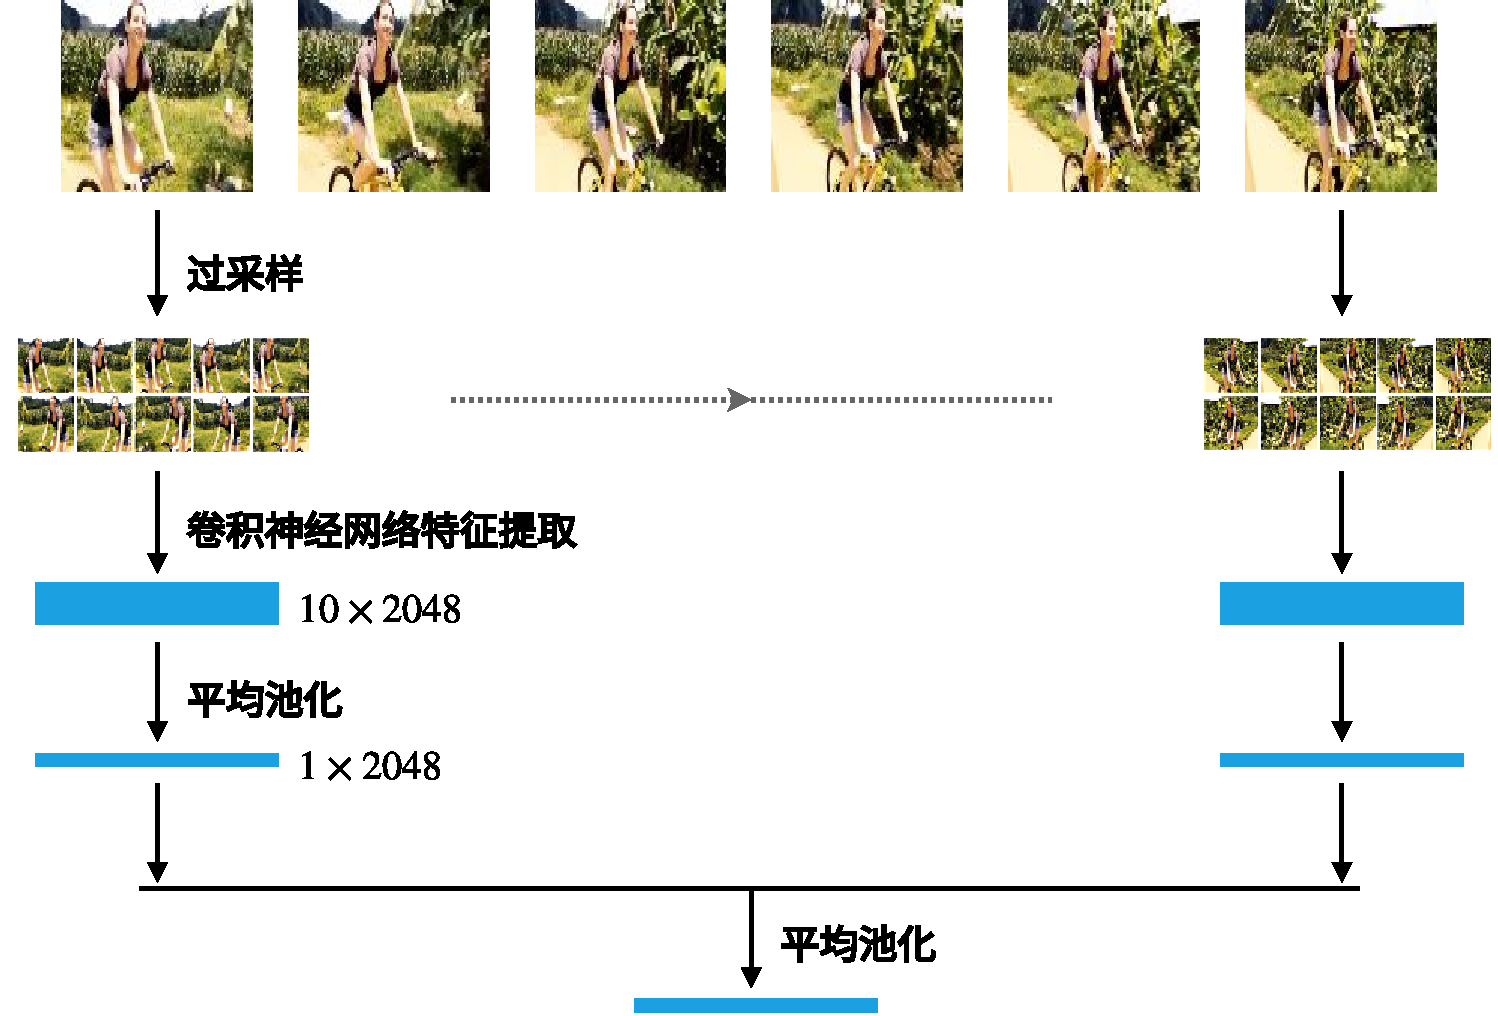
\includegraphics[width=\linewidth]{figures/video-cnn-feat}
    \caption[视频特征提取示例]{视频特征提取示例}
    \label{fig:video-cnn-feat}
\end{figure*}


\section{目标函数}




\section{公共空间表示}



,,
